% !TEX program = xelatex
% ¡Recuerda compilar con XeLaTeX o LuaLaTeX!
\documentclass{article}

% --- Cargar nuestro fichero de estilo ---
% Se asume que paper_style.sty está disponible o se usan paquetes estándar.
\usepackage{paper_style}

% --- PAQUETES PARA EL CONTENIDO DEL DOCUMENTO ---
\usepackage{graphicx}
\usepackage{subcaption}
\usepackage{amsmath}
\usepackage{booktabs}
\usepackage{geometry}
\usepackage{hyperref}
\usepackage{enumitem}
\usepackage{float}



% --- Información del Paper ---
\title{Informe: \\ Introducción a la Consola de Administración de AWS}
\author{
	Jordi Blasco Lozano \\
	\small Infraestructuras y Servicios Cloud \\
	\small Universidad de Alicante
}
\date{\today}

% --- Comienzo del Documento ---
\begin{document}
	
	\maketitle

	\begin{abstract}
	\noindent 
	

	\tableofcontents

	\newpage

	\section{Creación de la instancia base}

	\end{abstract}
	\begin{figure}[H]
	\centering
	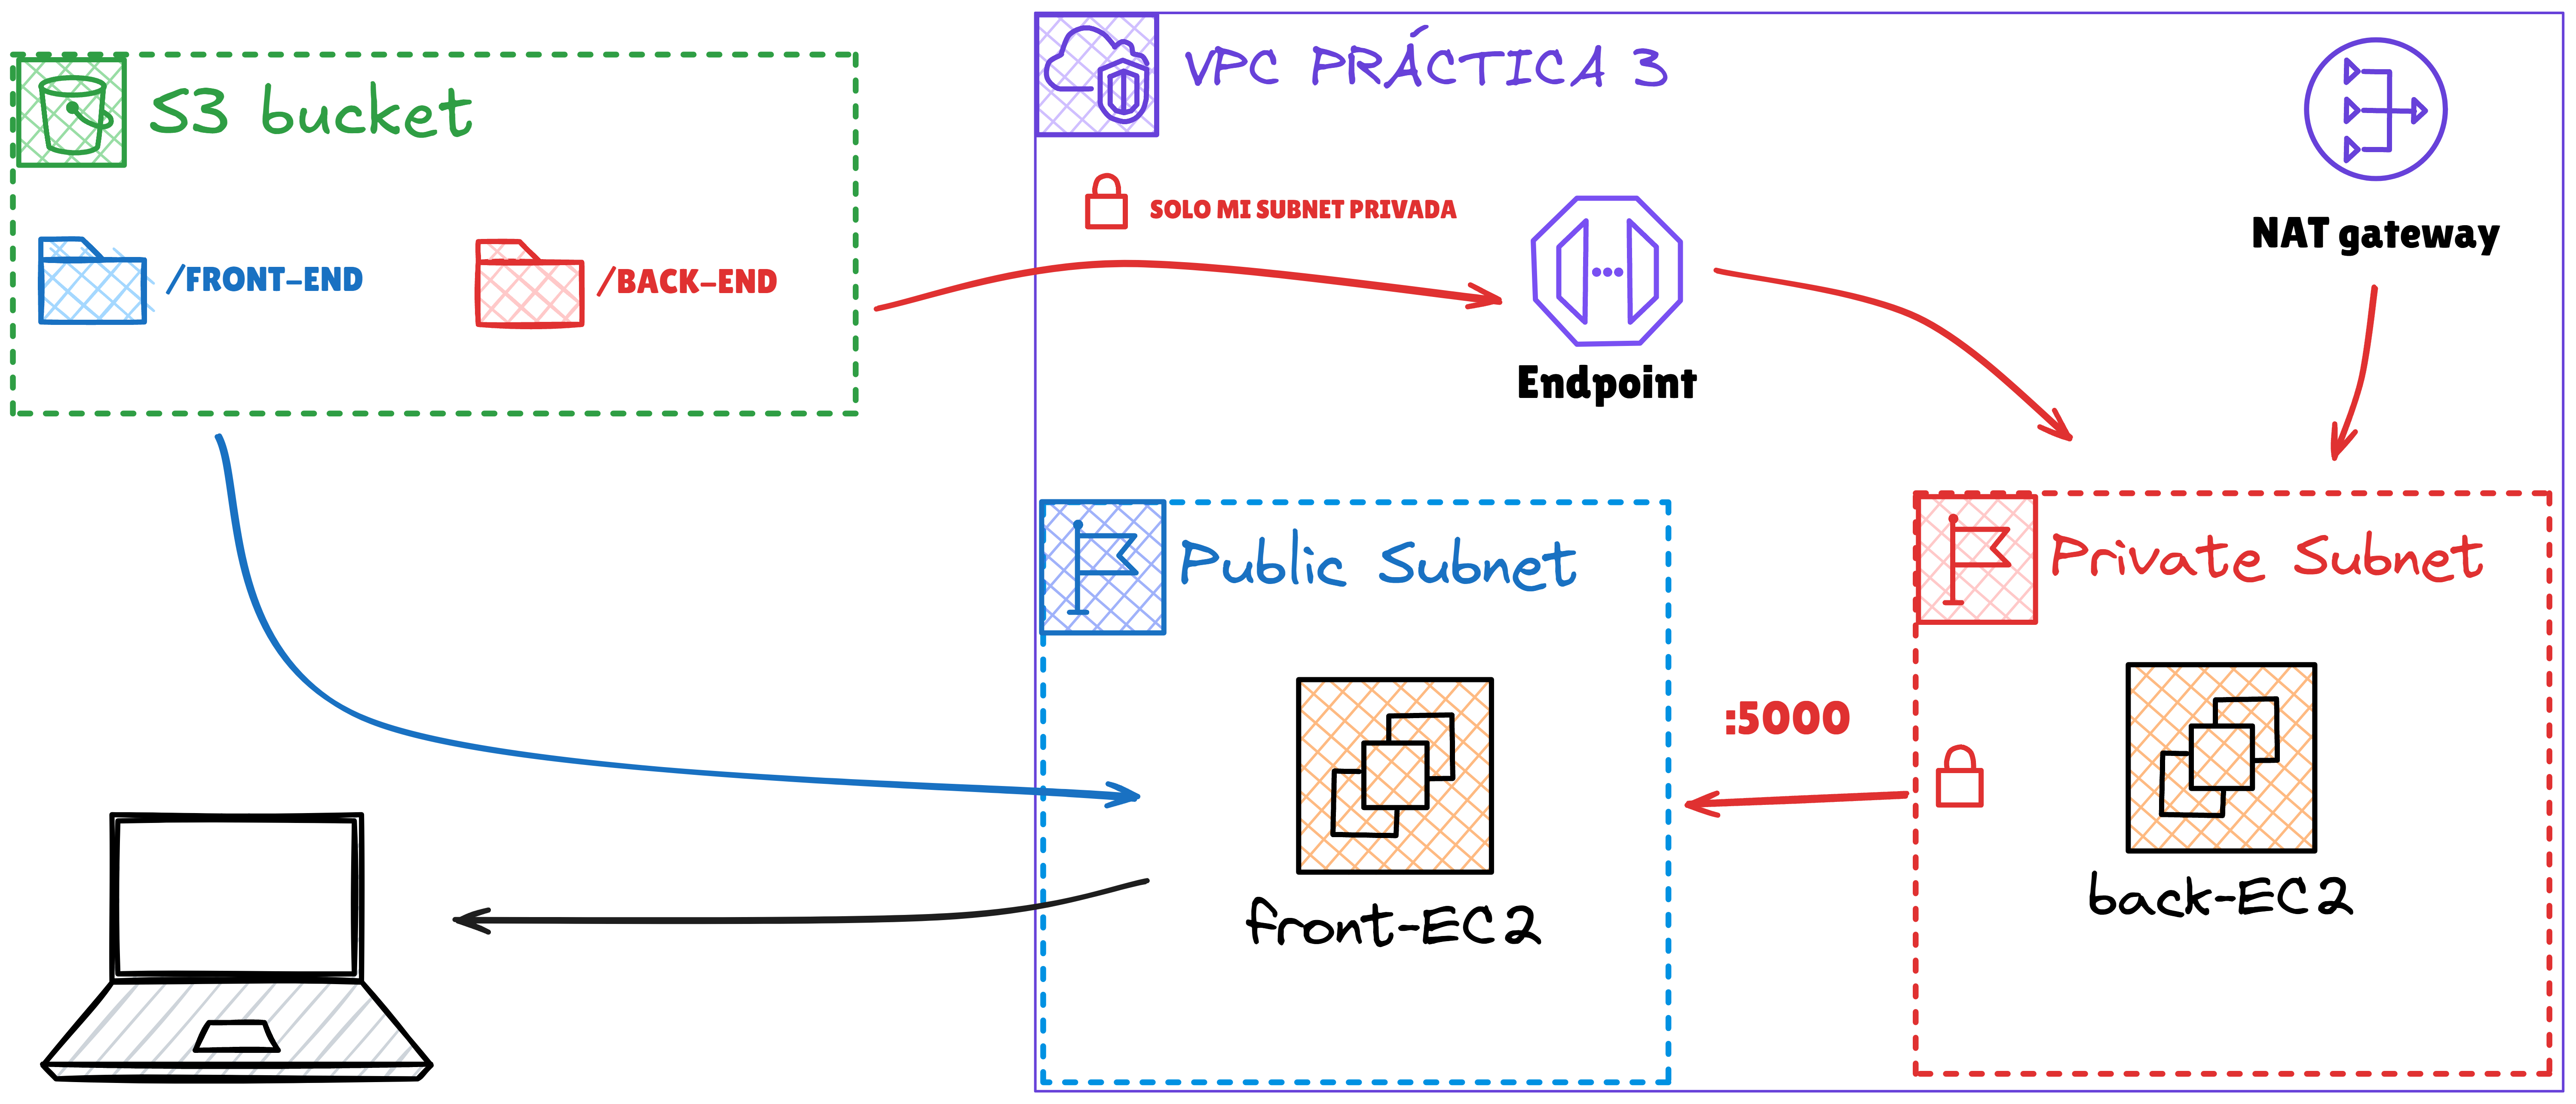
\includegraphics[width=0.95\textwidth]{esquema.png}
	\end{figure}

		

	\subsection{Configuración de red}

		
	
\newpage

	\subsection{Instalación de dependencias}

		Una vez tengamos la instancia creada deberemos de conectarnos a ella por ssh. Cuando estemos dentro de la instancia instalaremos httpd mediante el comando sudo yum install httpd. httpd es un servidor web Apache que utilizaremos para desplegar nuestro index.html.


\begin{lstlisting}[style=consola, language=bash, caption={Terminal, dependencias}]


\end{lstlisting}

\subsection{Archivo index.html}


\newpage